\documentclass{resume}
\usepackage{xcolor}
\definecolor{bronze}{rgb}{0.8, 0.5, 0.2}
\definecolor{gold}{rgb}{1.0, 0.84, 0.0}

\begin{document}
\fontfamily{ppl}\selectfont
\noindent 
\begin{tabularx}{\linewidth}{@{}m{0.75\textwidth} m{0\textwidth}@{}}
{
    \large {Markus Engelund Mathiasen} \newline
    \small{
        \clink{
            Email: \href{mailto:markusm@cs.au.dk}{markusm@cs.au.dk} \newline
             \href{https://github.com/markusmathiasen/}{GitHub}\hspace{2em}
             \href{https://www.linkedin.com/in/markus-mathiasen-5329a4303/}{LinkedIn}
        } \newline
    }
}
& 
{
    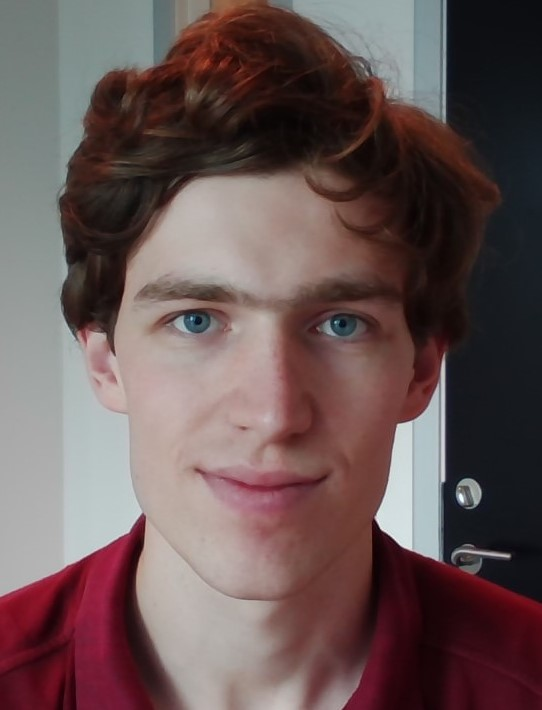
\includegraphics[height=4cm]{markus}
}
\end{tabularx}

\csection{Summary}{\small
    \begin{itemize}
        \item[] I am an ambitious student currently doing my PhD in computer science at Aarhus University. The PhD focuses on achieving better theoretical understanding of classic learning algorithms. During my bachelor's degree I have done extracurricular activities called Talent Track where I got to do interesting projects in the different research groups at the university. In my spare time, I like doing competitive programming, honing my skills by solving and implementing a variety of challenging algorithmic problems.
    \end{itemize}
}
\csection{Education}{\small
    \begin{itemize}
        \item \textbf{PhD in Computer Science (ongoing)\hfill{(2024-2028)}}\newline
        Aarhus University\\
        \textit{Project title:} Theoretical Understanding of Classic Learning Algorithms\\
        \textit{Advisor:} Kasper Green Larsen
        \item \textbf{Master in Computer Science (ongoing)\hfill{(2023-2026)}}\newline
        Aarhus University
        
        \item \textbf{Bachelor in Computer Science\hfill(2020-2023)}\newline
        Aarhus University\\
        \underline{Bachelor Thesis:}\\
        \textit{Title:} Graph Connectivity in the Semi-Streaming Model\\
        \textit{Advisor:} Chris Schwiegelshohn\\
        In this project, I looked at known results about how to decide whether a graph is connected or not in the semi-streaming model. I also looked at what we can do if we want the algorithm to be robust against an adaptive adversary.
    \end{itemize}
}

\csection{Publications}{\small
    \begin{itemize}
        \item \textbf{The Many Faces of Optimal Weak-to-Strong Learning\hfill(2024)}\\
        \textit{With:} Mikael Møller Høgsgaard and Kasper Green Larsen\\
        \textit{Conference:} Neural Information Processing Systems 2024 (NeurIPS)
    \end{itemize}
}

\csection{Teaching Experience}{\small
    \begin{itemize}
        \item \textbf{Teaching Assistant\hfill(2021-2024)}\newline
        I have been employed as teaching assistant at Aarhus University in the following bachelor activities on computer science.
        \begin{itemize}
            \item Algorithms and Data Structures\hfill(1 semester)
            \item Machine Learning\hfill(1 semester)
            \item Numerical Linear Algebra\hfill(1 semester)
            \item Programming Café\hfill(3 semesters)
            \item Programming Languages\hfill(2 semesters)
        \end{itemize}
        \item \textbf{Teacher at Dansk Datalogi Dyst\hfill(2021)}\newline
        I have made exercises and problems and done teaching at "Dansk Datalogi Dyst" where we train and select the best high school students to represent Denmark at the International Olympiad in Informatics.
    \end{itemize}
}

\csection{Talent Track}{\small
    \begin{itemize}
        \item[] Talent Track is an opportunity for bachelor students with a GPA of at least 10 to do extracurricular activities in the different research groups at the university on top of their normal studies. I have done extra work corresponding to 30 ECTS during my Bachelor. I have done the following projects the last four semesters of my bachelor:
        \item \textbf{Oblivious Data Structures\hfill(Spring 2023)}\newline
        Project with Peter Scholl where we looked at different data structures and how one can either make them oblivious, by using oblivious priority queues, or show that it is difficult by reducing them to ORAM.
        \item \textbf{Minimum DNF with Xor\hfill(Fall 2022)}\newline
        Project with Srikanth Srinivasan where we looked at a variation of the minimum DNF problem allowing xor in the literals. Specifically, we looked at why the reduction to set cover doesn't work in this variation, and alternative approaches to construct an approximation algorithm for this problem.
        \item \textbf{Micro WebAssembly in Coq\hfill(Spring 2022)}\newline
        Project with Jean Yves Alexis Pichon from the Logic \& Semantics research group where we looked at how to define Webassembly in Coq, constructing a syntactic and semantic type system for this, and proving their relation.
        \item \textbf{Randomized Algorithms\hfill(Fall 2021)}\newline
        Project with Kasper Green Larsen from the Algorithms research group where we looked at count sketch and how it can be used to find heavy hitters in a data stream efficiently.
    \end{itemize}
}
    
\csection{Competitive Programming}{\small
    \begin{itemize}
        \item \textbf{Danish Championship in Programming\hfill(2024)}\newline
        \textcolor{gold}{\textbf{Won}} the danish championship in programming for university students.
        \item \textbf{Northwestern Europe Regional Contest (NWERC)\hfill(2020-2024)}\newline
        Qualified for the team representing Aarhus University 5 times and won \textcolor{gold}{\textbf{gold medal}} in 2024.
        \item \textbf{Google Code Jam\hfill(2022)}\newline
        Advanced to round 3 (last round before world finals) and placed 435th in the world out of 32,000 participants in total.
        \item \textbf{International Olympiad in Informatics\hfill(2020)}\newline
        Qualified for the danish team.
        \item \textbf{Baltic Olympiad in Informatics\hfill(2020)}\newline
        Qualified for the danish team and won \textcolor{bronze}{\textbf{bronze medal}}.
    \end{itemize}
}

\end{document}